%%  设计封面

\begin{titlepage}
\centering %% 全部居中

    \rule{\textwidth}{1pt}   % The top horizontal rule


    %------------------------------------------------------------
    %    Title
    %------------------------------------------------------------
    
    %%  南航图标
    %\begin{figure}[H]
    %\centering
    %
\includegraphics[width=0.15\textwidth]{logo/nuaa-logo-black.pdf}
    %\end{figure}
    
    %%  南航艺术字体
    %\begin{figure}[H]
    %\centering
    %
\includegraphics[width=0.6\textwidth]{logo/nuaa-jianqi.pdf}
    %\end{figure}
    
    %%  竖直方向空位
    \vspace{0.01\textheight}
    
    {\Huge \textbf{机械设计基础课程设计计算说明书}}

    \rule{0.83\textwidth}{0.4pt}  % The short horizontal rule under title
    
    \flushleft{\large{\textbf{课题代号:}}{XXX}}  %%  在这更改你的课题代号
    
    \flushleft{\large{\textbf{数据代号:}}{XXX}}  %%  在这更改你的数据代号
     
    \flushleft{\large{\textbf{设计题目:}}{XXX装置}}  %%  在这更改你的装置名称
      
    \flushleft{\large{\textbf{传动简图:}}}  %%  在这更改你的传动简图
    \begin{figure}[H] %% H代表强制将此图插入在此处
        \centering
        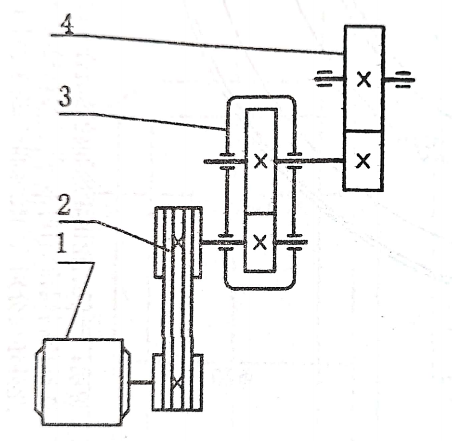
\includegraphics[width=0.3\textwidth]{figure/传动简图.png} 
        %% 自动搜寻figure目录下传动简图.png图片,width设置为0.3倍textwidth
        %  \caption{图片小标题设置栏}  封面图片可以不设小标题
        %\label{传动简图}  %%  标签设置为传动简图,后续可以用ref索引,封面图片没这个必要
    \end{figure}
    
    \flushleft{\large{\textbf{工作条件:}}{
    轻微振动载荷;双向传动;室内工作。。。(需修正)
    }}  %%  在这更改你的工作条件
    
    \flushleft{\large{\textbf{使用期限:}}{长期使用(需修正)}}  %%  在这更改你的使用期限
    
    \flushleft{\large{\textbf{设计工作量:}}{
    1、减速器装配图1张(A0);
    2、零件图:齿轮、输出轴各1张(A2),共计两份;
    3、计算说明书一份。
    }}  %%  设计工作量

    \vspace{0.02\textheight}  % Whitespace between the short horizontal rule and author

    %------------------------------------------------------------
    %    Author
    %------------------------------------------------------------
    
    \centering  %% 居中
    
    \large\textbf{学院:}\underline{\quad\quad{航空学院}\quad\quad}  %%  航空学院
    
    \large\textbf{专业:}\underline{\quad\quad{工程力学}\quad\quad}  %%  专业
    
    \large\textbf{姓名:}\underline{\quad\quad{XXX}\quad\quad}  %%  姓名
    
    \large\textbf{班级:}\underline{\quad\quad{0119xxxx}\quad\quad}  %%  班级
    
    \large\textbf{学号:}\underline{\quad\quad{0119xxxxxx}\quad\quad}  %%  学号
    
    \large\textbf{指导老师:}\underline{\quad\quad{XXX}\quad\quad}  %%  指导老师

    \vfill  % Whitespace between author and date
    
    \vspace{0.01\textwidth}

    {\Large \today}
    \vspace{0.01\textheight}  % Whitespace between date and bottom horizontal rule

    %------------------------------------------------------------
    %    Bottom rules
    %------------------------------------------------------------

    \rule{\textwidth}{1pt}  % The bottom horizontal rule


\end{titlepage}